% IEEE Access manuscript v1 (DRN-261027-01). Target changed from IEEE Sensors Journal to IEEE Access
% by user decision 2026-10-29. Brief: repo .claude_logs/paper/00_brief.md
% Template: ACCESS_latex_template_20260513 (ieeeaccess.cls md5 6e473d2a8652127c24e6e8af3d7a34f5),
%   provided by the user from the IEEE Template Selector on 2026-10-27; pristine copy ../templates/access-20260513/.
\documentclass{ieeeaccess}
\usepackage{cite}
\usepackage{amsmath,amssymb,amsfonts}
\usepackage{graphicx}
\usepackage{textcomp}
\usepackage{booktabs}
\usepackage{multirow}
\usepackage[hidelinks]{hyperref}
\definecolor{RED}{rgb}{1,0,0}% running heads may be uppercased, which turns `red' into `RED'
\newcommand{\todo}[1]{\textcolor{red}{[TODO: #1]}}
\newcommand{\missing}[1]{\textcolor{blue}{[MISSING: #1]}}
\newcommand{\td}{\textcolor{red}{todo}}% empty table cell, value pending
% table layout: every table uses \tabsetup (same font, same spacing) and spans exactly \columnwidth
\newcommand{\tabsetup}{\footnotesize\setlength{\tabcolsep}{2.5pt}\renewcommand{\arraystretch}{1.1}}
\newcommand{\tabnote}[1]{\par\vspace{3pt}\parbox{\columnwidth}{\raggedright\scriptsize #1}}
% placeholder frame for figures not drawn yet
\newcommand{\phbox}[2]{{\setlength{\fboxrule}{0.4pt}\setlength{\fboxsep}{3pt}%
  \fbox{\parbox[c][#1][c]{0.95\linewidth}{\centering\textcolor{red}{todo: #2}}}}}

\begin{document}
\history{Date of publication xxxx 00, 0000, date of current version xxxx 00, 0000.}
\doi{10.1109/ACCESS.2026.DOI}

\title{\todo{title}}
\author{\todo{authors and IEEE membership}}
\address[1]{\todo{affiliation and e-mail}}
\tfootnote{\todo{funding}}

\markboth
{\todo{Author et al.: short title}}
{\todo{Author et al.: short title}}

\corresp{\todo{corresponding author and e-mail}}

\begin{abstract}
% IEEE Access rule: one paragraph, 150-250 words, no abbreviations, footnotes, references, equations or tables.
% Numbers: headline.yaml (test 57.74, +1.03 vs DGFusion) and tasks/DRN-261019-03/analysis.md (validation missing-sensor score 57.85, +7.92).
Vehicles and robots fuse several sensors so that scene understanding survives when one sensor fails, yet the most accurate multimodal segmentation models lose much of their accuracy when a single input is missing. We investigate why. On a synthetic driving benchmark with camera, depth, event, and laser range inputs, we compare a leading fusion model that uses depth supervision with our own model that does not, under one evaluation protocol. Both depend heavily on depth: removing it costs 23 to 39 points of mean intersection over union, more at night than in daylight. When either model is also trained on synthetically degraded inputs, this dependence largely disappears, which indicates that it is learned from clean training data rather than caused by the fusion design. Building on this finding, we present a fusion model on a frozen vision foundation backbone with sensor-specific adapters, symmetric cross-sensor attention, and a high-resolution decoding path, trained with a clean pass and a degraded pass distilled from a clean teacher. The training needs no condition labels and adds no inference cost. The model reaches 57.7 mean intersection over union on the test set, one point above the best published fusion model, and 57.9 under the standard missing-sensor protocol on the validation set, eight points above the best published result. We further analyse sensor dependence across conditions, thin objects, and failure cases \todo{add one sentence on the real-sensor benchmarks once measured}.
\end{abstract}

\begin{keywords}
% IEEE Access template: three or four keywords or phrases, alphabetical order
Foundation models, missing modality, multimodal semantic segmentation, robustness, sensor fusion
\end{keywords}


\titlepgskip=-21pt

\maketitle

\section{Introduction}\label{sec:intro}
\PARstart{A}{utonomous} vehicles and mobile robots carry several sensors because each one fails in different conditions. A camera loses contrast at night and in fog, a depth estimate develops holes on reflective surfaces, an event camera goes silent on static scenes, and LiDAR returns thin out in rain and with distance. Multimodal semantic segmentation promises to cover these failures by fusing the sensors, so that the scene is still understood when one of them degrades.

Research on this problem has split into two tracks. The first track maximizes accuracy when all sensors are present~\cite{cmnext2023,cmx2023,stitchfusion2024,geminifusion2024,cafuser2025,dgfusion2026}. The second track measures and improves robustness when sensors are missing or noisy~\cite{magic2024,anyseg2024,rmmss2025,mmssbench2025,fuseadapt2026}. The two tracks rarely evaluate the same models under the same protocol. As a result, it is unclear whether the most accurate fusion models are also robust, and if they are not, what makes them fragile. A recent robustness benchmark~\cite{mmssbench2025} reports that several fusion models lose much of their accuracy when a sensor is removed, and it explains the differences by fusion design, contrasting RGB-centric, equal-contribution, and adaptive-selection architectures. Whether the design is in fact the cause has not been tested by holding the design fixed and changing only the training.

We study this question on three benchmarks with complementary sensor suites: DELIVER~\cite{cmnext2023} (RGB, depth, event, LiDAR), MUSES~\cite{muses2024} (RGB, event, LiDAR, radar), and MCubeS~\cite{mcubes2022} (RGB, polarization, near-infrared). We evaluate a leading accuracy-oriented model, DGFusion~\cite{dgfusion2026}, and our own fusion model under one protocol, and find that both rely heavily on depth on DELIVER: removing depth costs 23 to 39 points of mIoU, more in the dark than in daylight. DGFusion uses depth supervision, which might explain its dependence, but our model has no such supervision and shows the same pattern. When either model is trained with synthetically degraded inputs in addition to clean ones, the dependence largely disappears. The over-reliance is therefore learned from clean training data rather than built into a specific architecture.

Building on this finding, we present \ours{}, a fusion model on a frozen DINOv3 backbone with sensor-specific adapters, symmetric cross-modal attention, and a high-resolution decoding path, trained with a clean pass and a degraded pass that is distilled from a frozen clean teacher. The training scheme needs no condition or degradation labels and adds no inference cost. On DELIVER, \ours{} reaches 57.74 mIoU on the test set (mean of three seeds), 1.0 point above DGFusion, while reducing the depth over-reliance to a third or less, and it scores 57.85 under the standard missing-modality protocol on the validation set, 7.9 points above the best published result \todo{add the MUSES and MCubeS results once measured}.
% Sources: headline.yaml deliver.ours[0] (57.74, gap +1.03 vs DGFusion 56.71); tasks/DRN-261019-03/analysis.md (val EMM15 57.85 vs RMMSS 49.93, +7.92).

Our contributions are as follows.
\begin{itemize}
\item We show, with controlled comparisons on the same backbone and with re-trained baselines evaluated under one protocol, that the sensor over-reliance of accurate fusion models on DELIVER comes from clean training rather than from their architecture or supervision.
\item We combine a frozen foundation backbone with a two-pass training scheme and a high-resolution path into a single model that improves clean accuracy and robustness together, instead of trading one for the other.
\item We analyse per-sensor dependence across conditions, missing, partial, and noisy sensors, thin objects, and failure cases, and we report where the model still fails. \todo{state the code and checkpoint release}
\end{itemize}

\section{Related Work}\label{sec:related}
% Comparison table and audit for this section: repo .claude_logs/research/novelty-and-related-work.md and
% research/2026-10-20-structural-novelty-audit.md. Bibliography checked 2026-10-28 (notes/reference_check.md).

\subsection{Multimodal Fusion for Segmentation}
Early RGB-X segmentation fused one auxiliary sensor into an RGB stream, for example by cross-modal feature rectification~\cite{cmx2023} or by exchanging tokens between modality-specific transformers~\cite{tokenfusion2022}. CMNeXt~\cite{cmnext2023} generalized this to an arbitrary number of sensors with a hub that aggregates the auxiliary sensors before injecting them into RGB, and introduced DELIVER. Later work improved efficiency and accuracy with adapter-based early fusion~\cite{stitchfusion2024} and pixel-level token exchange~\cite{geminifusion2024}. CAFuser~\cite{cafuser2025} conditions the fusion on the scene condition inferred from the camera image, and DGFusion~\cite{dgfusion2026} uses depth, with depth supervision, to guide the fusion; both report leading results on DELIVER and MUSES. These methods are designed and evaluated with all sensors present. We re-train two of them with degraded inputs and show that their robustness depends mostly on training, not on their fusion design.

\subsection{Robustness to Missing and Degraded Sensors}
A second line of work trains models that tolerate missing sensors. MAGIC~\cite{magic2024,magicpp2024} treats all modalities equally and, during training, ranks modality features by their similarity to an aggregated feature. AnySeg~\cite{anyseg2024} names the problem unimodal bias, the over-reliance on a dominant, faster-to-learn modality, and reduces it by distilling a multimodal teacher into a student trained with random modality dropout; functional-entropy regularization~\cite{zheng2025entropy} targets the same bias. RMMSS~\cite{rmmss2025} combines prototype distillation with feature selection. A recent benchmark~\cite{mmssbench2025} standardized entire-missing, random-missing, and noisy-modality evaluations, which we adopt, and attributed robustness differences to fusion design. Our study differs from these works in its question and its controls: rather than proposing another robust architecture, we take the accuracy-leading fusion models, hold their architecture fixed, change only the training data, and measure how their dependence on each sensor changes across conditions. FuseAdapt~\cite{fuseadapt2026} adapts a frozen backbone with parameter-efficient fusion modules for missing modalities. Our training scheme uses the same building blocks as several of these methods, namely synthetic degradation and distillation from a clean teacher. We do not claim it as a new method; we use it to show where over-reliance comes from and to obtain a model that is both accurate and robust. Methods in this line usually skip a missing input, whereas the benchmark protocol replaces it with zeros; we keep the two families apart when comparing numbers.

\subsection{Adapting Frozen Foundation Models}
Vision foundation models are increasingly used as frozen encoders for dense prediction. The Segment Anything Model~\cite{sam2023} has been adapted to multimodal inputs with adapters that inject auxiliary-sensor features into the RGB stream~\cite{mmsamadapter2025} or with mixtures of LoRA experts~\cite{mlesam}, and MemorySAM~\cite{memorysam2025} reuses the memory mechanism of SAM~2 to fuse modalities. DINOv3~\cite{dinov3_2025} provides dense features and a segmentation adapter derived from ViT-Adapter~\cite{vitadapter2023}, which we reuse for our high-resolution path. Our backbone, LoRA adaptation~\cite{lora2022}, and query head~\cite{mask2former2022} follow this practice; we treat them as the platform for our study, not as contributions.

\section{Sensors, Benchmarks, and Protocol}\label{sec:sensors}
\todo{0.5 page: sensor physics and failure modes; DELIVER/MUSES/MCubeS; evaluation protocol}

\section{Method}\label{sec:method}
% Implementation facts below were read from the code on 2026-10-29: semseg/models/reliadino/{encoder,fusion,model,hires_adapter}.py,
% train_reliadino.py (two-pass loop l.1000-1110, _qaf_kd_kl l.283), semseg/datasets/degrade.py (TRAIN_OPS l.159),
% config configs/lecun-deliver_rgbdel_P46_c3only_seed20260821_screen40_A2hires.yaml.

Fig.~\ref{fig:arch} summarizes \ours{}. The model keeps a single foundation backbone frozen and shares it across all sensors, so that every sensor is read with the same visual vocabulary. It adds a small number of trained components around the backbone: sensor-specific low-rank adapters, a symmetric cross-modal fusion, a decoder with a high-resolution path, and two complementary heads. Training uses every batch twice, once clean and once with synthetic sensor degradation, and distills a frozen clean-trained teacher into the degraded pass.

\begin{figure*}[t]
\centering
% Source: figures/src/fig_arch_standalone.tex + latex/figures/fig_arch.tex (TikZ), built by build.sh.
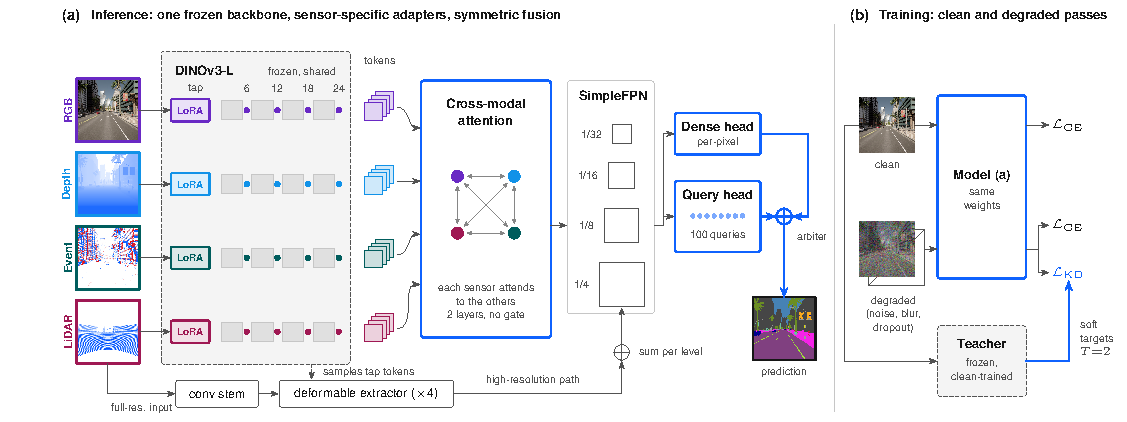
\includegraphics[width=\textwidth]{figures/fig_arch.pdf}
\caption{Overview of \ours{}. (a) Each sensor passes through the same frozen DINOv3-L with its own LoRA adapter; tokens from four depths are fused by symmetric cross-modal attention, decoded by a SimpleFPN augmented with a high-resolution path, and classified by a dense head and a query head combined by an arbiter. (b) Every batch is used twice: a clean pass and a synthetically degraded pass, the latter also distilled from a frozen teacher trained on clean data. Blue outlines mark trained components; dashed boxes are frozen. The scene and the prediction are a DELIVER test image and the output of our model. \todo{draft drawn by the paper session; redraw per notes/figure\_guide.md}}
\label{fig:arch}
\end{figure*}

\subsection{Frozen Backbone with Sensor-Specific Adapters}
Let $x_s$ denote the input of sensor $s\in\{1,\dots,S\}$, converted to a three-channel image (Section~\ref{sec:exp}). Every $x_s$ is processed by the same DINOv3 ViT-L/16 backbone~\cite{dinov3_2025}, whose weights are frozen. To let each sensor adapt the shared features to its own statistics, we attach a separate low-rank adapter (LoRA)~\cite{lora2022} of rank 8 to the attention projections of the backbone for each sensor. Instead of reading only the last layer, we take the token maps after blocks 6, 12, 18, and 24, so that the decoder receives both low-level and semantic evidence; each of the four maps is projected by a sensor-specific $1\times1$ layer. The result is a stride-16 token set $T_s$ for every sensor.

\subsection{Symmetric Cross-Modal Fusion}
Many fusion designs nominate RGB as the primary stream and inject the other sensors into it~\cite{cmx2023,mmsamadapter2025}, which makes the model fragile exactly when RGB fails. We instead treat the sensors symmetrically. In each of two fusion layers, the tokens of sensor $s$ form the queries of a multi-head attention whose keys and values are the tokens of all other sensors,
\begin{equation}
T_s \leftarrow T_s + \mathrm{MHA}\big(T_s,\ [T_{s'}]_{s'\neq s},\ [T_{s'}]_{s'\neq s}\big),
\end{equation}
followed by a feed-forward layer. No sensor is privileged, and the attention has no gate and receives no external reliability signal. The fused tokens of all sensors are merged by a gated MLP into one stride-16 feature map $F$. In addition, a per-class sensor router inherited from earlier versions of our model adds a zero-initialized residual term to the logits. \todo{decide with the method session how to describe the router (MODEL.ROUTER = per-class reliability-anchored modality router, fusion.py:64) and whether it needs its own ablation row; earlier internal measurement: about +0.1 mIoU}

\subsection{Decoder with a High-Resolution Path}
A SimpleFPN~\cite{vitadapter2023} turns $F$ into a feature pyramid at strides 4, 8, 16, and 32. Because every level is interpolated from stride-16 tokens, structures thinner than a token, such as poles and pedestrians at a distance, are poorly represented. We therefore add a high-resolution path that follows the adapter used in the official DINOv3 segmentation code~\cite{dinov3_2025,vitadapter2023}. A convolutional stem with weights shared across sensors (and a sensor-specific $1\times1$ projection) extracts multi-scale features from the raw inputs. Four deformable-attention extractors then let these convolutional queries sample semantic evidence from the four tapped token maps. Unlike the original adapter, we use only the extractors and do not inject anything back into the backbone, which stays untouched. The path's output is added to the FPN levels without a gate. We regard this path as an engineering complement taken from prior work, not as a contribution, and we analyze where its gain comes from in Section~\ref{sec:analysis}.

\subsection{Dense and Query Heads}
Two heads read the pyramid. A dense convolutional head classifies every pixel at stride 4. A Mask2Former-style query head~\cite{mask2former2022} with 100 queries and six decoder layers predicts class scores and masks, which are converted into per-pixel class scores $Q$. An arbiter combines the two with a learned per-class weight $\lambda_k$ that is initialized at zero,
\begin{equation}
\ell_k(p) = D_k(p) + \lambda_k\, Q_k(p),
\end{equation}
so that the query head contributes only where it helps the dense prediction.

\subsection{Two-Pass Training with Teacher Distillation}
Our analysis in Section~\ref{sec:analysis} shows that over-reliance on one sensor is learned from clean training data. We therefore change the training signal rather than the architecture. Every batch $(x, y)$ is used twice. The clean pass computes the segmentation loss $\mathcal{L}_{\mathrm{seg}}(f(x), y)$. The degraded pass builds $\tilde{x}$ by corrupting each sensor of each sample independently with probability 0.5; one fifth of the corrupted sensors are removed entirely (zero-filled), and the rest receive one operator drawn from a sensor-specific set: patch dropout, blur, gain and gamma changes, colour shift (RGB), depth holes (depth), beam dropout (LiDAR), and resolution loss (event). The corruption strength follows a curriculum that rises from 0.3 to 0.6 and 1.0 of its maximum at epochs 0, 10, and 20. Gaussian and salt-and-pepper noise are deliberately excluded from training so that the noise evaluation tests generalization to unseen corruption.

The degraded pass is supervised by the labels and by a frozen teacher $g$, a model of the same architecture without the high-resolution path that was trained on clean data only. The teacher sees the clean input, and its soft predictions are distilled into the degraded pass:
\begin{equation}
\begin{split}
\mathcal{L} ={} & \mathcal{L}_{\mathrm{seg}}(f(x), y) + \mathcal{L}_{\mathrm{seg}}(f(\tilde{x}), y)\\
& + \alpha\, T^2\, \mathrm{KL}\!\left(\sigma\!\left(\tfrac{g(x)}{T}\right) \Big\|\, \sigma\!\left(\tfrac{f(\tilde{x})}{T}\right)\right),
\end{split}
\end{equation}
with $\alpha=0.5$ and $T=2$, where $\sigma$ is the softmax over classes and the Kullback--Leibler divergence is averaged over pixels. The scheme needs no condition labels and no degradation labels, and it adds no computation at inference. Its parts are known: clean-teacher distillation and synthetic dropout appear in robust multimodal segmentation~\cite{anyseg2024,rmmss2025}. Our point is not a new loss but the evidence that this change of training signal, and not the architecture, removes the sensor over-reliance (Section~\ref{sec:analysis}).

\section{Experiments}\label{sec:exp}
\subsection{Implementation Details}
% Source: configs/lecun-deliver_rgbdel_P46_c3only_seed20260821_screen40_A2hires.yaml (TRAIN, OPTIMIZER, SCHEDULER, LOSS, MODEL.M2F, MODEL.P46.C3_PROTO, MODEL.P39).
All sensors are converted to three-channel images as in CMNeXt~\cite{cmnext2023}. We train for 40 epochs with AdamW (learning rate $6\times10^{-4}$, weight decay 0.01), a polynomial schedule with power 0.9, and a 10-epoch warm-up, on $768\times768$ crops with an effective batch size of 16 obtained by gradient accumulation. We use the data augmentation of DGFusion~\cite{dgfusion2026} so that both models see the same augmented images. The segmentation loss combines online hard-example cross-entropy~\cite{ohem2016} on the dense head with the set-prediction loss of the query head (weight 0.5, with deep supervision) and three auxiliary terms inherited from earlier versions of our model: an auxiliary cross-entropy on the fusion output, a class-prototype contrastive term (weight 0.1), and a variance-covariance regularizer on the fused tokens; we list them for reproducibility and do not claim them as contributions \todo{one-line ablation or citation for the auxiliary terms, or move to the supplement}. The frozen teacher is the same architecture without the high-resolution path, trained for 200 epochs on clean data. Unless noted, we report the mean of three seeds and the best seed; ablations use one seed.

\subsection{Comparison with Prior Fusion Models}
Table~\ref{tab:deliver} compares \ours{} with fusion models on DELIVER. We list only methods evaluated under the protocol that reports test-split mIoU, because DELIVER results in the literature are reported under at least three different protocols and are not comparable across them. \ours{} reaches 57.74 test mIoU on average over three seeds and 58.61 for the best seed, 1.0 and 1.9 points above DGFusion. Its margin over MM SAM-adapter, which uses only RGB and depth, is 0.4 points on average \todo{val 3-seed mean; val comparison with CAFuser-CAA 68.79}. Tables~\ref{tab:muses} and~\ref{tab:mcubes} report the same model on the real MUSES and MCubeS benchmarks \todo{results pending: MUSES four-sensor model, MCubeS transfer}.
% Sources: headline.yaml deliver.ours[0] (57.74 / best 58.61; gap +1.03 / +1.90 vs DGFusion 56.71; +0.39 / +1.26 vs MM SAM-adapter 57.35);
% protocol clusters: repo research/novelty-and-related-work.md l.74-85 (secondary; cite original tables).


% Layout rule (user 2026-10-27): no \resizebox on tables. Every table uses \tabsetup and
% tabular* at \columnwidth, so all tables share one font size and none overflows the column.

% ---------------------------------------------------------------------------
% Table 1. DELIVER, all four sensors.
% Baselines: only the test-unified cluster (DGFusion protocol, "mIoU-test").
%   Do NOT mix with the high cluster (CMNeXt 66.30 / MemorySAM 65.38).
%   Candidate values for todo cells are in repo research/novelty-and-related-work.md:78-83
%   (secondary copy) -> must be taken from each original paper table, cite table+page.
% Ours: experiments/headline.yaml benchmarks.deliver.ours[0] (A2, 3 seeds, legal v2, test@1024).
%   val 3-seed mean is not recorded in headline.yaml (only seed903 69.86) -> todo.
% ---------------------------------------------------------------------------
\begin{table}[t]
\caption{DELIVER (RGB, depth, event, LiDAR), mIoU (\%).}
\label{tab:deliver}
\centering\tabsetup
\begin{tabular*}{\columnwidth}{@{\extracolsep{\fill}}lllcc@{}}
\toprule
Method & Backbone & Sensors & val & test \\
\midrule
CMNeXt~\td & \td & RGB-D-E-L & \td & \td \\
StitchFusion~\td & \td & RGB-D-E-L & \td & \td \\
GeminiFusion~\td & \td & RGB-D-E-L & \td & \td \\
CAFuser~\td & \td & RGB-D-E-L & \td & \td \\
CAFuser-CAA~\td & \td & RGB-D-E-L & 68.79 & \td \\
DGFusion~\td & Swin-T & RGB-D-E-L & \td & 56.71 \\
\midrule
\multicolumn{5}{@{}l}{\emph{Fewer sensors (secondary comparison)}} \\
MM SAM-adapter~\td & \td & RGB-D & 69.60 & 57.35 \\
\midrule
Ours (3-seed mean) & DINOv3-L & RGB-D-E-L & \td & 57.74 \\
Ours (best seed) & DINOv3-L & RGB-D-E-L & \td & 58.61 \\
\bottomrule
\end{tabular*}
\tabnote{\textcolor{red}{todo: original table/page per baseline; protocol (val-best checkpoint, 1024, nearest-exact label resampling); DINOv3-L is frozen.}}
\end{table}

% ---------------------------------------------------------------------------
% Table 2. MUSES, four sensors (RGB, event, LiDAR, radar). Only the 4-sensor A2 model
%   (user 2026-09-29; 3-sensor numbers 79.788 etc. are not used).
% Ours: DRN-261019-02 (queued) -> todo. Baselines: headline.yaml benchmarks.muses.
% ---------------------------------------------------------------------------
\begin{table}[t]
\caption{MUSES, official evaluation, mIoU (\%).}
\label{tab:muses}
\centering\tabsetup
\begin{tabular*}{\columnwidth}{@{\extracolsep{\fill}}lllcc@{}}
\toprule
Method & Backbone & Sensors & val & test \\
\midrule
CAFuser~\td & \td & \td & \td & \td \\
DGFusion~\td & \td & \td & \td & 79.5 \\
\midrule
\multicolumn{5}{@{}l}{\emph{Camera only or fewer sensors (secondary comparison)}} \\
GtA~\td & \td & RGB & \td & 82.39 \\
MM SAM-adapter~\td & \td & RGB-L & \td & 81.07 \\
\midrule
Ours & DINOv3-L & RGB-E-L-R & \td & \td \\
\bottomrule
\end{tabular*}
\end{table}

% ---------------------------------------------------------------------------
% Table 3. MCubeS (RGB, AoLP, DoLP, NIR). Ours: DRN-261017-02 (A2 transfer, 2 seeds) -> todo.
%   58.07 in headline.yaml is the previous generation (P39.1 recipe), not the paper model.
% ---------------------------------------------------------------------------
\begin{table}[t]
\caption{MCubeS (RGB, AoLP, DoLP, NIR), test mIoU (\%).}
\label{tab:mcubes}
\centering\tabsetup
\begin{tabular*}{\columnwidth}{@{\extracolsep{\fill}}llc@{}}
\toprule
Method & Backbone & test \\
\midrule
Mul-VMamba~\td & \td & 54.65 \\
StitchFusion~\td & \td & 55.9 \\
\midrule
Ours & DINOv3-L & \td \\
\bottomrule
\end{tabular*}
\end{table}

\subsection{Robustness to Missing and Degraded Sensors}
Table~\ref{tab:robust} and Fig.~\ref{fig:robust} evaluate all models under the same missing-sensor and noise protocol. Under the public benchmark definition on the validation set, \ours{} scores 57.85 EMM, 7.9 points above the best published result, and it keeps 61 to 66 mIoU when a quarter to three quarters of a sensor's pixels are missing. On the test set, the official DGFusion weights fall to 31.5 EMM and to 5.5 mIoU under the strongest noise, which shows how much the accuracy-oriented models depend on complete inputs. Re-training DGFusion and CAFuser with our synthetic degradation raises their EMM to 45.5 and 46.5 without changing their architecture. \ours{} reaches 48.7 EMM while keeping the highest clean accuracy, so it does not trade accuracy for robustness, and it retains 47.9 mIoU under the strongest noise, which was never seen during training.
% Sources: tasks/DRN-261019-03/analysis.md (val EMM15 57.85, RMM 65.53/63.35/61.28, test EMM15 48.66, NM 47.85);
% judgment-ledger 2026-10-01 row (DGFusion (a) EMM 31.53, NM .20 5.52; (b) EMM 45.52); current.md (4) CAFuser (b) EMM 46.50.

When only one sensor is available (Fig.~\ref{fig:robust}b), the official DGFusion collapses to 12.1 mIoU with RGB alone and to 1.2 and 3.2 with event or LiDAR alone, while still reaching 43.1 with depth alone. Training with degraded inputs lifts every single-sensor score, most strongly for RGB (49.0 for the re-trained DGFusion and 53.9 for our model without the high-resolution path). Sensor dependence, in other words, follows the training data.
% Source: judgment-ledger 2026-10-01 row (single-sensor EMM subsets; Q2 3 seeds 53.9/46.0/31.0/22.9).

% ---------------------------------------------------------------------------
% Table 4. Missing and degraded sensors on DELIVER.
% (a) Benchmark family (2503.18445 definition: normalize then zero-fill), val.
%     Ours: tasks/DRN-261019-03/analysis.md (A2 3 seeds, mm_eval_v2): EMM15 57.85,
%     RMM15 r.25/.5/.75 65.53/63.35/61.28. RMMSS EMM 49.93: same doc / headline.yaml note.
% (b) Same protocol, our measurement on test (61 cases, 1897 images):
%     DGFusion (a) official weights / (b) degradation retrained: experiments/judgment-ledger.md
%       2026-10-01 row (DRN-260930-02). CAFuser (b): status/current.md (4) "CAFuser (b) 10-04".
%     "w/o two-pass" = E1 40ep screen 3 seeds, EMM 40.01: ledger 2026-10-01 row.
%     "w/o high-res" = Q2 3 seeds, "Ours" = A2 3 seeds: tasks/DRN-261019-03/analysis.md
%       (Q2 NM is 2 seeds for s902/s903 plus s821 where available; see that table).
%     Depth/RGB partial-drop columns omitted: Q2 values disagree between ledger 10-01 (3 seeds:
%     0.98/2.04/2.64) and DRN-261019-03 (2 seeds: 0.47/1.05/1.36) -> resolve before use.
% Families that skip missing inputs (AnySeg, RMMSS, RobustSeg 1a, FuseAdapt) are not mixed here.
% ---------------------------------------------------------------------------
\begin{table}[t]
\caption{Robustness to missing and degraded sensors on DELIVER, mIoU (\%).}
\label{tab:robust}
\centering\tabsetup
\begin{tabular*}{\columnwidth}{@{\extracolsep{\fill}}lccccc@{}}
\toprule
\multicolumn{6}{@{}l}{\emph{(a) Public missing-modality benchmark, val}} \\
Method & EMM & RMM .25 & RMM .50 & RMM .75 & \\
\midrule
RMMSS~\td & 49.93 & \td & \td & \td & \\
Ours (3 seeds) & 57.85 & 65.53 & 63.35 & 61.28 & \\
\midrule
\multicolumn{6}{@{}l}{\emph{(b) Same protocol for all models, test}} \\
Method & Clean & EMM & S\&P .05 & S\&P .10 & S\&P .20 \\
\midrule
DGFusion (official) & 55.68 & 31.53 & 37.97 & 16.71 & 5.52 \\
DGFusion (retrained$^{\dagger}$) & 54.77 & 45.52 & 48.89 & 40.51 & 23.34 \\
CAFuser (retrained$^{\dagger}$) & 55.79 & 46.50 & \td & \td & \td \\
Ours w/o two-pass & \td & 40.01 & \td & \td & \td \\
Ours w/o high-res & 56.59 & 48.06 & 53.25 & 51.64 & 48.79 \\
Ours & 57.74 & 48.66 & 53.11 & 51.36 & 47.85 \\
\bottomrule
\end{tabular*}
\tabnote{$^{\dagger}$Retrained with the same synthetic degradation. Ours: mean of 3 seeds; baselines: single runs.
\textcolor{red}{todo: define EMM (mean over 15 sensor subsets), RMM (random drop ratio), S\&P noise.}}
\end{table}

% ---------------------------------------------------------------------------
% Fig. robust (data plot). Source numbers and provenance: figures/src/make_data_figs.py (fig_robust).
% ---------------------------------------------------------------------------
\begin{figure}[t]
\centering
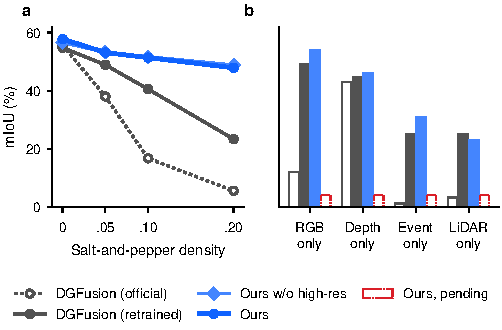
\includegraphics[width=\columnwidth]{figures/fig_robust.pdf}
\caption{Robustness on DELIVER test under one protocol. (a) Salt-and-pepper noise applied to every sensor. (b) Only one sensor available (the other three zero-filled). Ours: mean of three seeds; DGFusion: single runs, official weights or retrained with the same synthetic degradation. \todo{(b) full-model values pending.}}
\label{fig:robust}
\end{figure}

\subsection{Qualitative Results}
Figs.~\ref{fig:failure_scenarios} and~\ref{fig:adverse} show scenes selected by a fixed rule: among all test images, those where the gap between our model and the best baseline is largest, at most one scene per condition and map \todo{describe what the scenes show once selected}.

% Fig. sensor-failure scenarios (main qualitative figure). Needs per-image predictions of
% DGFusion (official), DGFusion/CAFuser (retrained) and ours under missing/noisy sensors
% -> analysis request inbox 20261027-182054 item 2.
\begin{figure*}[t]
\centering
\phbox{5.2cm}{Fig.~3 when a sensor fails: rows = depth missing / RGB missing / LiDAR+event missing / RGB with heavy noise; columns = affected input, ground truth, DGFusion (official), DGFusion (retrained), CAFuser (retrained), ours; error pixels in one colour}
\caption{\todo{caption; state the scene-selection rule (top differences between ours and the best baseline, one scene per condition, no repeated map)}}
\label{fig:failure_scenarios}
\end{figure*}

% Fig. adverse conditions with all sensors present, DELIVER (synthetic) + MUSES (real).
% DELIVER dumps exist: NAS analysis_logs/native_axis_baseline_20261016/{dgfusion,cafuserb}_test1024,
% a2_test1024_dump_20261016/s821 -> analysis request inbox 20261027-182054 item 1. MUSES: item 3.
\begin{figure*}[t]
\centering
\phbox{4.6cm}{Fig.~4 adverse conditions, all sensors present: DELIVER night / fog / rain / low exposure and MUSES real night / snow / fog; columns = RGB, ground truth, DGFusion, CAFuser, ours; zoomed crops where the baselines miss objects}
\caption{\todo{caption; state the scene-selection rule}}
\label{fig:adverse}
\end{figure*}

\subsection{Accuracy per Condition}
Table~\ref{tab:condition} breaks clean test accuracy down by condition \todo{text after the per-condition numbers arrive (analysis request 20261028-183826 item 1)}.

% ---------------------------------------------------------------------------
% Table 5. Clean mIoU per condition on DELIVER test (new 2026-10-28, user: 10-page budget).
% Source: to be computed by analysis from the same dumps as Fig. adverse (inbox addendum).
% ---------------------------------------------------------------------------
\begin{table}[t]
\caption{DELIVER test mIoU (\%) per condition, all sensors present.}
\label{tab:condition}
\centering\tabsetup
\begin{tabular*}{\columnwidth}{@{\extracolsep{\fill}}lccccccc@{}}
\toprule
Model & Sun & Cloud & Rain & Fog & Night & Low exp. & All \\
\midrule
DGFusion (official) & \td & \td & \td & \td & \td & \td & 55.68 \\
DGFusion (retrained$^{\dagger}$) & \td & \td & \td & \td & \td & \td & 54.77 \\
CAFuser (retrained$^{\dagger}$) & \td & \td & \td & \td & \td & \td & 55.79 \\
Ours w/o high-res & \td & \td & \td & \td & \td & \td & 56.59 \\
Ours & \td & \td & \td & \td & \td & \td & 57.74 \\
\bottomrule
\end{tabular*}
\tabnote{$^{\dagger}$Retrained with synthetic degradation. All: same values as Table~\ref{tab:robust}(b) clean column.}
\end{table}

\subsection{Ablation}
Table~\ref{tab:ablation} builds the model up from a frozen DINOv3-L with LoRA on RGB alone and then removes one component at a time from the full model, all with the same seed and schedule. The frozen backbone alone reaches 55.14 mIoU with RGB, already within 1.6 points of DGFusion with four sensors, so a large part of the accuracy comes from the foundation model. Adding the other three sensors with cross-modal attention and the query head gives 55.94, the two-pass training with distillation adds 1.8 points (57.73), and the high-resolution path adds 0.9 (58.61). Removing cross-modal attention or the query head costs 0.85 and 0.72 points, respectively. Replacing the sensor-specific adapters with one shared adapter does not reduce clean accuracy (58.84) \todo{robustness of the shared variant and the degradation-pass and distillation rows (L5, L6) pending}.
% Sources: judgment-ledger 2026-10-28 rows DRN-261020-08/-09/-10/-12 (seed 821, legal v2 test@1024);
% E1 screen s821 55.94: status/current.md (4); Q2/A2 s821 57.73/58.61: tasks/DRN-261019-03/analysis.md.

% ---------------------------------------------------------------------------
% Table 6. Ablation on DELIVER test, seed 821, 40 epochs, legal v2.
% RGB-only 55.14 = judgment-ledger 2026-10-28 DRN-261020-08 (adopted as ladder row).
% L1 shared LoRA 58.84, L2 mean fusion 57.76, L4 dense head only 57.89 = judgment-ledger 2026-10-28
%   rows DRN-261020-09/-10/-12 (test@1024 legal v2, seed 821). L2 also removes the trunk expansion
%   (code constraint, ledger note). L5 DRN-261020-13 / L6 -14 evaluating; mean-fusion ladder -07 running.
% mean fusion = DRN-261020-07 (evaluating). E1 screen s821 55.94 = status/current.md (4).
% Q2 s821 57.73 / EMM 48.68 and A2 s821 58.61 / EMM 49.12 = tasks/DRN-261019-03/analysis.md.
% Leave-one-out: L1 DRN-261020-09, L2 -10, L4 -12, L5 -13, L6 -14 (queued). L3 withdrawn.
% ---------------------------------------------------------------------------
\begin{table}[t]
\caption{Ablation on DELIVER test (one seed, 40 epochs), mIoU (\%).}
\label{tab:ablation}
\centering\tabsetup
\begin{tabular*}{\columnwidth}{@{\extracolsep{\fill}}lcc@{}}
\toprule
Configuration & Clean & EMM \\
\midrule
\multicolumn{3}{@{}l}{\emph{Building up}} \\
Frozen DINOv3-L + LoRA, RGB only & 55.14 & -- \\
+ depth, event, LiDAR (mean fusion) & \td & \td \\
+ cross-modal attention, query head & 55.94 & \td \\
+ two-pass training, distillation & 57.73 & 48.68 \\
+ high-res path (full model) & 58.61 & 49.12 \\
\midrule
\multicolumn{3}{@{}l}{\emph{Removing one component from the full model}} \\
$-$ sensor-specific LoRA (one shared) & 58.84 & \td \\
$-$ cross-modal attention (mean fusion)$^{*}$ & 57.76 & \td \\
$-$ query head and arbiter & 57.89 & \td \\
$-$ degradation pass & \td & \td \\
$-$ teacher distillation & \td & \td \\
\bottomrule
\end{tabular*}
\tabnote{$^{*}$Also removes the trunk expansion. \textcolor{red}{todo: EMM column for ablation runs; decision on shared LoRA pending its robustness test.}}
\end{table}

\subsection{Computational Cost}
Table~\ref{tab:cost} reports parameters, operations, latency, and memory at the evaluation resolution \todo{numbers pending (DRN-261027-02); the two-pass training doubles the forward passes during training but adds nothing at inference}.

% ---------------------------------------------------------------------------
% Table 7. Cost on DELIVER at 1024, same GPU. DRN-261027-02 (queued) -> all todo.
% ---------------------------------------------------------------------------
\begin{table}[t]
\caption{Computational cost on DELIVER at $1024\times1024$.}
\label{tab:cost}
\centering\tabsetup
\begin{tabular*}{\columnwidth}{@{\extracolsep{\fill}}lccccc@{}}
\toprule
Model & Params & Trainable & GFLOPs & Latency & Memory \\
 & (M) & (M) & & (ms) & (GB) \\
\midrule
DGFusion & \td & \td & \td & \td & \td \\
CAFuser & \td & \td & \td & \td & \td \\
Ours w/o high-res & \td & \td & \td & \td & \td \\
Ours & \td & \td & \td & \td & \td \\
\bottomrule
\end{tabular*}
\end{table}

\section{Analysis}\label{sec:analysis}

% Figure plan: notes/figure_guide.md §2. Qualitative scenes come from recorded dumps only
% (path + md5 in the figure source note) and the selection rule is stated in the caption.

\subsection{Where Sensor Over-Reliance Comes From}
A fusion model can lean on one sensor because its architecture or supervision favours that sensor, or because the training data make that sensor sufficient. DGFusion~\cite{dgfusion2026} is a useful test case: it adds depth supervision to its fusion, and removing depth costs the official model 23 to 37 points depending on the condition (Fig.~\ref{fig:dependence}). If the depth supervision caused this dependence, a model without it should behave differently.

Our own architecture trained only on clean data, which has no depth supervision, shows the same pattern: removing depth costs 23.5 to 38.7 points, and the cost grows from sun to low exposure exactly as for DGFusion. The same architecture trained with the two-pass scheme loses only 3.9 points in sun, 10.1 at night, and 13.4 under low exposure. The effect also holds across architectures. When we re-train DGFusion with the same synthetic degradation, removing depth entirely costs 4.7 points instead of 33.3, and the EMM score rises from 31.5 to 45.5 (Table~\ref{tab:robust}).
% Sources: judgment-ledger 2026-09-30 row (E1 confirmed, Q2 s821, DGFusion official, oracle_cond probe);
% judgment-ledger 2026-10-01 row (DGFusion (a)->(b): depth fully missing -33.3 -> -4.7, EMM 31.53 -> 45.52).

We conclude that, on DELIVER, the dependence on depth is a property of clean training rather than of a particular fusion design or supervision. A plausible reason is that DELIVER renders depth without noise or holes, so clean training finds a shortcut that real depth sensors would not offer. Two caveats bound this conclusion. The clean-only model was trained for 200 epochs and the two-pass model for 40, and the DGFusion curve was measured on the test split while ours were measured on validation \todo{remove the second caveat once all curves are re-measured on one split}. A complementary observation is that our clean-only model is already less sensitive to salt-and-pepper noise than the re-trained DGFusion; we therefore attribute part of the noise robustness to the frozen DINOv3 backbone rather than to our training \todo{state the measured drops (ledger 2026-10-01: E1 3.09/5.73/11.22 vs DGFusion retrained 5.9/14.3/31.4) after checking that the definitions match}.

\begin{figure}[t]
\centering
% Source numbers and provenance: figures/src/make_data_figs.py (fig_dependence). Full table: sections/supp_tables.tex (Table S1).
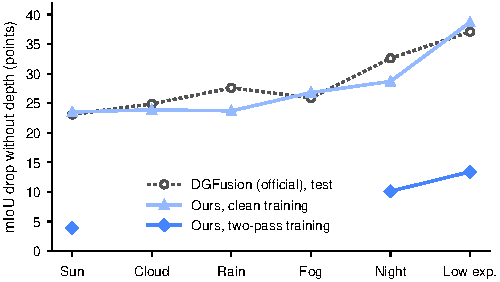
\includegraphics[width=\columnwidth]{figures/fig_dependence.pdf}
\caption{Drop in mIoU when depth is removed, per condition. A model trained only on clean data relies on depth as heavily as DGFusion, whose design adds depth supervision; two-pass training reduces the drop to a third or less with the same architecture. DGFusion was measured on test, the other curves on val. \todo{re-measure all curves on one split; add the full model and the retrained baselines.}}
\label{fig:dependence}
\end{figure}

\subsection{What the High-Resolution Path Adds}
The high-resolution path raises clean test mIoU by 1.15 points on average over three seeds (from 56.59 to 57.74; Table~\ref{tab:ablation}). Fig.~\ref{fig:thin} shows where the gain comes from. Averaged over the three seeds, Static gains 10.4 points, Pedestrian 3.8, TrafficSign 3.1, and Pole 2.1, and the four thin classes gain 3.0 points together. The gain comes mainly from recall: for Pole the recall rises from 0.75 to 0.78 and for Pedestrian from 0.89 to 0.90 \todo{confirm these recall values (two seeds, NAS analysis\_logs/a2\_thin\_anatomy\_20261018/summary.md) through the analysis session before citing}. Two classes lose: TrafficLight by 4.1 points and RailTrack by 7.2. RailTrack varies strongly between seeds even without the path (58.5, 32.6, and 45.1 for the three seeds), so we do not interpret its change. The TrafficLight loss, in contrast, is systematic and is analysed next.
% Sources: per-class 3-seed CSV .claude_logs/experiments/analysis/DRN-261018-01/a2_vs_q2_perclass_3seed.csv (d_mean3 column);
% thin-4 mean +3.04 and 24-class Δ +1.50: tasks/DRN-261018-01/analysis.md.

\begin{figure}[t]
\centering
% Source: .claude_logs/experiments/analysis/DRN-261018-01/a2_vs_q2_perclass_3seed.csv (3 seeds, legal v2 test 1024);
% plot: figures/src/make_data_figs.py (fig_thin).
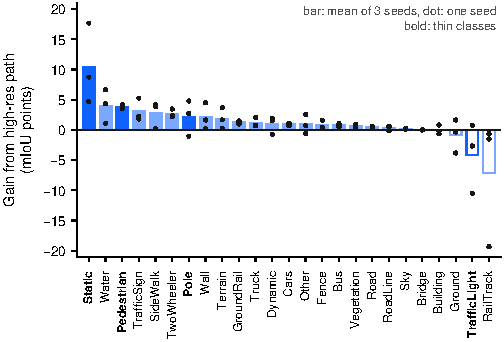
\includegraphics[width=\columnwidth]{figures/fig_thin.pdf}
\caption{Per-class gain of the high-resolution path on DELIVER test, paired by seed (full model minus the same model without the path). Thin classes gain most; TrafficLight and RailTrack lose and vary strongly across seeds. \todo{add zoomed crops of thin objects (Q2 dumps on yeon).}}
\label{fig:thin}
\end{figure}

\subsection{Failure Case: Posters Read as Traffic Lights}
With the high-resolution path, the recall of TrafficLight rises (0.80 to 0.85) but its precision falls (0.46 to 0.41) \todo{same confirmation as above}. Fig.~\ref{fig:failure} shows where the extra false positives appear. In the scenes with the largest increase, billboards and posters, labelled as \emph{Other}, are painted as traffic lights, and in one rainy scene a traffic sign is. The two classes share fine structure, a small bright rectangular shape on a pole or a wall, but differ in context. Because the high-resolution features are added to every pyramid level without a gate, fine detail reaches the dense per-pixel classifier directly, and the classifier can follow the detail without enough context. This mechanism is a hypothesis that our measurements are consistent with but do not prove; we discuss a remedy in Section~\ref{sec:conclusion}.
% Source: NAS analysis_logs/a2_tl_fp_scenes_20261022/README.md (4 scenes; A2 vs Q2 TrafficLight FP pixels
% 15258 vs 3620, 13705 vs 3752, 10304 vs 2008, 12229 vs 9008; selection rule: top-20 by A2 FP - Q2 FP, no repeated condition).

\begin{figure}[t]
\centering
% Assets: NAS analysis_logs/a2_tl_fp_scenes_20261022 (4 scenes, README.md has the selection rule).
\phbox{4.2cm}{limitation: posters and signs predicted as traffic light (2 of the 4 recorded scenes; RGB, ground truth, ours, error map)}
\caption{\todo{caption; selection rule from the scene README: among the 20 test images where our model adds the most TrafficLight false positives relative to the model without the high-resolution path, one scene per condition.}}
\label{fig:failure}
\end{figure}

\subsection{Limitations}
First, DELIVER is synthetic, and its complete depth is the reason the shortcut exists; the size of the effect on real depth sensors remains to be measured, and MUSES does not contain depth. Second, all our runs use a 40-epoch schedule and three seeds, while the baselines are single runs, so differences below about one point should not be over-read. Third, the high-resolution path makes the model slightly more sensitive to heavy pixel noise and to partial loss of depth or RGB than the same model without it (Table~\ref{tab:robust}); a likely cause is that its convolutional stem sees raw pixels, which we have not yet verified. Fourth, a single shared LoRA reached the same clean accuracy as sensor-specific adapters in one seed (Table~\ref{tab:ablation}); \todo{update once the shared-LoRA robustness test decides which variant is the paper model}.

\section{Conclusion}\label{sec:conclusion}
We asked why accurate multimodal segmentation models fail when one sensor degrades. Controlled comparisons on DELIVER showed that their heavy dependence on depth is learned from clean training data: it appears in our model without depth supervision as strongly as in DGFusion with it, and it largely disappears in both architectures when degraded inputs are added to training. Built on this finding, \ours{} combines a frozen DINOv3 backbone, symmetric fusion, and a high-resolution path with two-pass training, and improves clean accuracy and robustness together on DELIVER \todo{and on MUSES and MCubeS, once measured}. The analysis also exposes what remains: the high-resolution path recovers thin objects but lets fine detail mislead the per-pixel classifier, as in posters read as traffic lights, which suggests routing fine detail to mask prediction rather than to per-pixel classification. Measuring the same dependence on real depth sensors is the next step that our synthetic-data findings call for.


% bibliography enabled once sections contain \cite (empty thebibliography breaks the build)
%\bibliographystyle{IEEEtran}
%\bibliography{IEEEabrv,references}

% IEEE Access requires author biographies with photos at the end.
\begin{IEEEbiographynophoto}{\todo{Author name}}
\todo{biography (photo 1 in $\times$ 1.25 in)}
\end{IEEEbiographynophoto}

\EOD
\end{document}
